%(BEGIN_QUESTION)
% Copyright 2010, Tony R. Kuphaldt, released under the Creative Commons Attribution License (v 1.0)
% This means you may do almost anything with this work of mine, so long as you give me proper credit

\vbox{\hrule \hbox{\strut \vrule{} {\bf Desktop Process exercise} \vrule} \hrule}

The concept of {\it feedback control} is much easier to grasp when you have the luxury of experimenting with a real control system.  In this program, one of the ways you will gain hands-on experience with control systems is to experiment with a miniature process that fits on a desktop.

A simple diagram of this ``Desktop Process'' is shown here, where a single-loop controller controls the speed of a DC electric motor:

$$\includegraphics[width=15.5cm]{i04150x01.eps}$$

The motor receives its power from the Variable-Speed Drive (VSD), and reports shaft speed to the controller by means of a tachogenerator (``tach'') which generates a DC voltage proportional to shaft speed.

\vskip 10pt

Experiment with this ``Desktop Process'' in the following ways:

\begin{itemize}
\item{} Place the controller into manual mode and adjust the controller's output to see how the motor spins (and how its speed is registered on the controller's process variable display).
\vskip 10pt 
\item{} Place the controller into automatic mode and adjust the controller's setpoint to see how well the motor speed tracks setpoint.  How closely does the motor speed come to being equal with setpoint?  How long does it take the motor speed to equalize with setpoint (if it ever does)?
\vskip 10pt 
\item{} Place the controller into manual mode with the motor spinning at approximately 50\% speed, then touch the motor shaft with your finger to ``load'' it down.
\vskip 10pt 
\item{} Place the controller into automatic mode with the motor spinning at approximately 50\% speed, then touch the motor shaft with your finger to ``load'' it down.  How does the automatic-mode response differ from the manual-mode response?  In which mode is the motor easiest for you to slow down?
\end{itemize}

\vskip 20pt \vbox{\hrule \hbox{\strut \vrule{} {\bf Suggestions for Socratic discussion} \vrule} \hrule}

\begin{itemize}
\item{} In your own words, explain the purpose of the controller having a ``manual'' mode.  If a controller's job is to exert automatic control on a process, why would it ever be useful to turn that automatic option off and go to manual mode?
\end{itemize}

\underbar{file i04150}
%(END_QUESTION)




%(BEGIN_ANSWER)


%(END_ANSWER)





%(BEGIN_NOTES)

\vskip 20pt \vbox{\hrule \hbox{\strut \vrule{} {\bf Virtual Troubleshooting} \vrule} \hrule}

This question is a good candidate for a ``Virtual Troubleshooting'' exercise.  Presenting the diagram to students, you first imagine in your own mind a particular fault in the system.  Then, you present one or more symptoms of that fault (something noticeable by an operator or other user of the system).  Students then propose various diagnostic tests to perform on this system to identify the nature and location of the fault, as though they were technicians trying to troubleshoot the problem.  Your job is to tell them what the result(s) would be for each of the proposed diagnostic tests, documenting those results where all the students can see.

During and after the exercise, it is good to ask students follow-up questions such as:

\begin{itemize}
\item{} What does the result of the last diagnostic test tell you about the fault?
\item{} Suppose the results of the last diagnostic test were different.  What then would that result tell you about the fault?
\item{} Is the last diagnostic test the best one we could do?
\item{} What would be the ideal order of tests, to diagnose the problem in as few steps as possible?
\end{itemize}


%INDEX% Desktop Process: introduction to feedback control

%(END_NOTES)


